\begin{frame}{Constrained Geometric Approximation}
\begin{columns}
  \begin{column}{.65\textwidth}
    \begin{itemize}
    \item \textbf{Goal}:\\
    For an extremely simple robot with:
    \begin{itemize}
    \item computation limitations
    \item moving and sensing uncertainties
    \end{itemize}
    represent and reason about uncertainty in its own states efficiently.\\
    \item \textbf{Basic Idea}:\\
    Explicitly represent what the robot knows as an information state (\textit{I-state}).
    \item \textbf{Intuition}:\\
    Accelerate time-consuming operations by maintaining only an \textcolor[rgb]{1.00,0.00,0.00}{over-approximation} of the true
    I-state, and constraining this approximation
    to have a simple geometric form.\\
    \end{itemize}
  \end{column}
  \begin{column}{.35\textwidth}
    \begin{figure}
    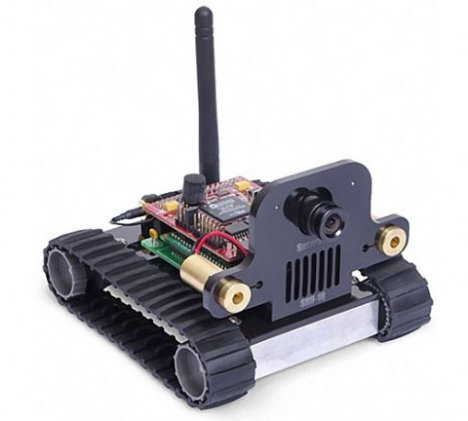
\includegraphics[scale=0.2]{figs/srvq.jpg}
    \end{figure}
    SRV-1 Surveyor Robot
  \end{column}
\end{columns}
\end{frame}